\chapter[LAMBDA]{ARQUITETURA LAMBDA}

A Arquitetura Lambda é uma abordagem para processar dados em uma plataforma
que lida com uma grande massa de dados, e surge como um caminho alternativo
a outras arquiteturas mais antigas, como a incremental com \textit{sharding}
\cite{marz2015}.

De maneira geral, a Arquitetura Lambda é composta de três camadas: a camada
\textit{batch}, que constantemente processa uma grande quantidade de dados e
demora razoavelmente em seu processamento; a camada \textit{serving},
responsável por disponibilizar os resultados do processamento; e a camada
\textit{speed}, responsável por atuar enquanto a camada \textit{batch} está
ocupada processando \cite{marz2015}. Cada uma destas camadas é implementada
utilizando algoritmos e ferramentas específicas, de modo que certas ferramentas
são mais apropriadas em certos contextos.

\begin{figure}
  \centering
    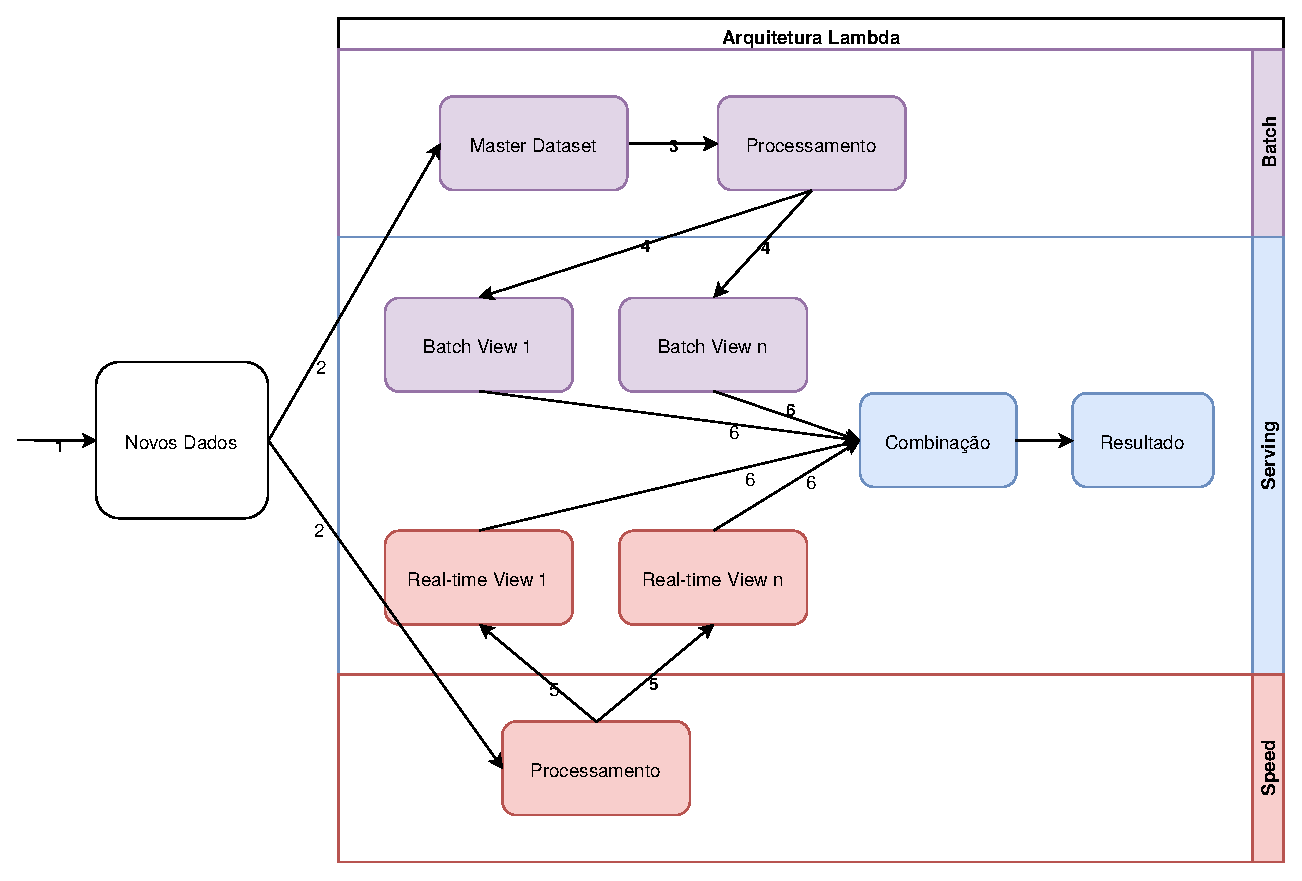
\includegraphics[width=\textwidth]{figuras/lambda-lifecycle.eps}
  \caption{Ciclo de vida na Arquitetura Lambda.}
  \label{fig:lambda-lifecycle}
\end{figure}

Um ciclo de vida típico da Arquitetura Lambda pode ser acompanhado na figura
\ref{fig:lambda-lifecycle}, e têm seu início com a (i) chegada
de novos dados, que serão então (ii) transmitidos tanto para a camada
\textit{batch} quanto para a camada \textit{speed}. A camada \textit{batch}
(iii) anexa os novos dados, e os processa, (iv) gerando assim
\textit{batch views}, que são enviados para a camada \textit{serving}. O mesmo
dado que foi enviado para a camada \textit{batch}, no passo (i), também foi
enviado para a camada \textit{speed}, (v) onde será processado com menor latência,
por só levar em conta dados recentes, e gerando \textit{real-time views}. 
Caso uma consulta seja feita, ocorre então uma (vi) soma entre os resultados
dos \textit{batch views} e \textit{real-time views} \cite{marz2015}.

A Arquitetura Lambda garante sua resiliência através da \textit{isolação de
complexidade}, que é obtida graças a sua separação entre camadas \textit{batch}
e \textit{speed}. A resiliência ocorre pois uma vez que os resultados são
processados na camada \textit{batch}, os resultados da camada \textit{speed}
podem ser descartados. Essa técnica é importante pois a transmissão pode
criar inconsistências, pois um dado que não vai ser levado em conta no
processamento pode ser necessário; contudo, essa inconsistência será corrigida
num lote futuro que será processado pela camada \textit{batch}, e os resultados
da camada \textit{speed} (que está incoerente) serão descartados
\cite{marz2015}.

Neste capítulo serão apresentados detalhes importantes da Arquitetura Lambda, e
possibilidades de tecnologias a serem utilizadas. Todas as tecnologias
levantadas são código livre, de boa qualidade, e utilizadas por gigantes da
industria.

\section{BATCH LAYER}

Responsável pelo processamento de uma grande massa de dados, e tendo como ponto
fraco a alta latência, a camada \textit{batch} é responsável por gerenciar e
criar um \textit{master dataset} (um lote de informação, imutável, e que só
pode \textbf{receber} anexos) \cite{marz2015}. Os dados na camada \textit{batch}
são então imutáveis, de modo que, caso uma mudança seja necessária, o dado que
carece alteração não sofre transformações, permanecendo inalterado, mas um novo
dado com as alterações é inserido no lote \cite{marz2015}. Por fim, a camada
\textit{batch} fará o pré-processamento dos dados presentes no
\textit{master dataset}, disponibilizando-os em \textit{batch views}.

\subsection{Tecnologias}

\begin{itemize}
    \item \textbf{Apache Hadoop MapReduce}: \textit{framework} para processamento
de dados distribuído, que utiliza abstrações simples. O Hadoop conta com sistema
de gerenciamento de arquivo nativo através do Hadoop HDFS. Em cenários onde a
latência não precisa ser tão baixa, o MapReduce é uma opção bem sólida, e
utilizado pelos mais altos escalões da
industria \footnote{\url{https://wiki.apache.org/hadoop/PoweredBy}}.

    \item \textbf{Apache Spark}: utilizando principalmente o módulo Spark SQL
\footnote{\url{http://spark.apache.org/sql/}}, o Spark trás uma nova abordagem
para a camada \textit{batch}, pois utiliza menos o disco e mais a memória,
através de uma abordagem chamada de \textit{micro-batch} \cite{arsalan2014}.
O Spark não conta com um sistema de gerenciamento de arquivo nativo, e pode
ser utilizado em conjunto com o Hadoop HDFS. Em um contexto onde menor latência
é preferida o Spark é a solução ideal.

\end{itemize}

\begin{table}[]
    \centering
    \caption[Resultados da Sort Benchmark 2014, categoria GraySort]{Resultados da Sort Benchmark 2014, categoria GraySort. Fonte: Databricks\footnotemark\\.}
    \label{tab:graysort2014results}
    \resizebox{\textwidth}{!}{%
        \begin{tabular}{|l|l|l|l|}
            \hline
             & \textbf{Hadoop MRRecord}      & \textbf{SparkRecord}             & \textbf{Spark1 PB}               \\ \hline
             Data Size                    & 102.5 TB                      & 100 TB                           & 1000 TB                          \\ \hline
             Elapsed Time                 & 72 mins                       & 23 mins                          & 234 mins                         \\ \hline
             \# Nodes                     & 2100                          & 206                              & 190                              \\ \hline
             \# Cores                     & 50400 physical                & 6592 virtualized                 & 6080 virtualized                 \\ \hline
             Cluster disk throughput      & 3150 GB/s(est.)               & 618 GB/s                         & 570 GB/s                         \\ \hline
             Sort Benchmark Daytona Rules & Yes                           & Yes                              & No                               \\ \hline
             Network                      & dedicated data center, 10Gbps & virtualized (EC2) 10Gbps network & virtualized (EC2) 10Gbps network \\ \hline
             \textbf{Sort rate}           & \textbf{1.42 TB/min}          & \textbf{4.27 TB/min}             & \textbf{4.27 TB/min}             \\ \hline
             \textbf{Sort rate/node}      & \textbf{0.67 GB/min}          & \textbf{20.7 GB/min}             & \textbf{22.5 GB/min}             \\ \hline
        \end{tabular}
    }
\end{table}

\footnotetext{\url{https://databricks.com/blog/2014/11/05/spark-officially-sets-a-new-record-in-large-scale-sorting.html}}

Em uma competição chamada Sort
Benchmark \footnote{\url{http://sortbenchmark.org/}}, na categoria GraySort,
que tem como objetivo mensurar quão rápido uma tecnologia ordena 100 TB de
dados, o Spark apresentou uma performance três vezes maior que o Hadoop
MapReduce, utilizando dez vezes menos recursos. Os resultados podem ser
conferidos na tabela \ref{tab:graysort2014results}.

\section{SPEED LAYER}

Durante o processamento da camada \textit{batch}, novos dados podem ser
inseridos. Caso somente a \textit{batch} processasse, esses novos dados não
seriam levados em conta em novas consultas; este problema é resolvido
na Arquitetura Lambda através da camada \textit{speed}, que é capaz de
processar dados em baixa latência \cite{marz2015}.

O diferencial entre a camada \textit{speed} e a camada \textit{batch} com
relação a performance e latência, se deve ao fato da \textit{speed} só
considerar a massa de dados que foi inserida após a camada \textit{batch}
ter começado a processar. Como a massa de dados é então muito menor, a
latência das operações também é mais baixa. A abordagem para processamento
também é diferente: a camada \textit{batch} analisa um lote de dados de uma
vez, enquanto a camada \textit{speed} processa dados conforme eles chegam.
Essa abordagem utilizada pela camada \textit{speed} é chamada de transmissão,
e funciona bem com mecanismos de passagem de mensagem \cite{marz2015}.
O fato da camada \textit{speed} utilizar transmissão, faz com que o uso de
banco de dados que suportem escrita aleatória seja necessário \cite{marz2015},
diferentemente da camada \textit{batch}. Por fim, a camada \textit{speed}
condensa o processamento feito em \textit{real-time views}, que são análogas
as \textit{batch views}, mas feitas somente com os dados processados via
transmissão.

%tradução de streaming pra transmissão fica ok?


\subsection{Tecnologias}

\begin{itemize}
    \item \textbf{Apache Spark}: através do módulo Spark Streaming
\footnote{\url{http://spark.apache.org/streaming/}}, é capaz de fornecer a
camada \textit{speed} na Arquitetura Lambda. Uma das vantagens de se utilizar
o Spark é então a complexidade reduzida, por usar uma única tecnologia e
código base nas duas camadas da Arquitetura Lambda. O Spark Streaming ainda
loteia eventos antes de processá-los, o que aumenta o tempo de processamento
em relação a outras soluções, contudo, essa abordagem faz com que a massa de
dados que ele possa processar seja maior
\footnote{\url{http://xinhstechblog.blogspot.com.br/2014/06/storm-vs-spark-streaming-side-by-side.html}}.

    \item \textbf{Apache Storm}: solução distribuída com foco em processamento
em tempo real. Tem a vantagem de poder ser utilizado com qualquer linguagem de
programação, e, por processar eventos no momento em que estes chegam
\footnote{\url{http://xinhstechblog.blogspot.com.br/2014/06/storm-vs-spark-streaming-side-by-side.html}}.

\end{itemize}

\section{SERVING LAYER}

Após os \textit{master datasets} da camada \textit{batch} serem criados ou
extendidos, \textit{batch views} são disponibilizados para a camada
\textit{serving}. A camada \textit{serving} torna possível a possibilidade de
fazer consultas a massa de dados processada, e de fazer leituras aleatórias
\cite{marz2015}. Conforme novos lotes são processados, a camada \textit{serving}
automaticamente troca os lotes antigos pelos novos, garantindo atualização dos
resultados.

Uma característica interessante desta camada é que, embora ela precise ser
capaz de fazer leitura aleatória, substituição de \textit{batch views}, e
responder consultas rapidamente (pois os dados já terão sido processados),
esta camada não precisa ser capaz de fazer escrita aleatória \cite{marz2015}.
Esse fato reduz substancialmente a complexidade necessária para as tecnologias
desta camada, de modo que só precisem se preocupar com os outros requisitos
citados.

\subsection{Tecnologias}

\begin{itemize}
    \item ElephantDB
    \item Apache Cassandra
\end{itemize}

\section{BROKER}

Existem várias abordagens para prover a comunicação entre diferentes módulos e
tecnologias, e, um desses modos é através da passagem de mensagem. O
\textit{broker} é uma peça chave na Arquitetura Lambda, pois ele será o
responsável por trocar informações via transmissão com a camada
\textit{speed}, e, em outros casos, também servir de meio para a comunicação
entre outros módulos \cite{marz2015}.

Uma abstração que facilita a compreensão dessa abordagem, e do papel do
\textit{broker}, se baseia em pensá-lo como um sistema de correios. Os
microserviços como abstração de pessoas, decidem qual canal utilizarão,
através das \textbf{conexões} e das \textbf{filas}. Caso um serviço queira
enviar e receber mensagens sobre um determinado assunto, ele deve se registrar
em um \textbf{tópico} no \textit{broker}. Por fim, quando uma mensagem for
receptada pelo \textit{broker}, ele o entregará a todos os serviços registrados
naquele tópico, como um carteiro.

\subsection{Tecnologias}

\begin{itemize}
    \item \textbf{RabbitMQ}: usado por empresas como a Cisco, Instagram,
New York Times, dentre outros \footnote{\url{https://www.rabbitmq.com/}}, e
com suporte para diversas linguagens \cite{zaitsev2014}, apresenta como
principal característica o fato de ser feito em Erlang, e, assim, utilizar
o poder da BEAM, possuindo alto desempenho, tolerância a falhas e processamento
distribuído>

    \item \textbf{Apache Kafka}:
\end{itemize}


